%descomente abaixo para imprimir no formato de livro.
%\documentclass[ruledheader,11pt]{abnt-fisica9}
\documentclass[12pt]{abnt-fisica11}% opcao padrao, comente se desejar opcao livro
\usepackage[utf8]{inputenc}
\usepackage{algorithm}
\usepackage{algpseudocode}
\usepackage{color, colortbl}
\usepackage{tikz}
\usepackage[brazil]{babel}
\usepackage{amsfonts}
\usepackage{multicol}
\usepackage{euscript}
\usepackage{float}
\usepackage{amsmath}
\usepackage{tikz,tkz-euclide}
\usetikzlibrary{arrows,calc,patterns}
\usepackage{epsfig,fisica-ufc11,graphicx,cite}
\usepackage{array}
\newcolumntype{P}[1]{>{\centering\arraybackslash}p{#1}}
	
\definecolor{Gray}{gray}{0.9}

\usepackage[num]{abntex2cite11}
\usepackage{mathrsfs}
% Use o bibtex
\newcommand{\mycomment}[1]{}
\usetikzlibrary{calc}
\tikzset{make origin horizontal center of bounding box/.style={%
execute at end picture={%
\path let \p1=(current bounding box.west),\p2=(current bounding box.east)
in ({-max(-1*\x1,\x2)},\y1) ({max(-1*\x1,\x2)},\y1);
}}}
% Opção alf para citações tipo (Author, data)


% descomente se quizer no padrão de livro papel b5:
%\estilobook

% se for  compiliar em pdflatex (aceita o brasao em pdf e gera o pdf ao inves do dvi)descomente a linha abaixo
\DeclareMathAlphabet{\mathpzc}{OT1}{pzc}{m}{it}
\pdflatextrue
\begin{document}

% essas informacoes do codigo CIP você consegue indo na biblioteca central
\codigocip{S185r}{CDD 530}%

\Ilustracao{1}% escolha 0 se não tiver ilustrações, 1 para ilustrações em petro e branco e 2 para ilustrações coloridas

\Tipo{1}%Escolha 0 para monografias, 1 para qualificação de mestrado, 2 para dissertação de mestrado,  3 para 
%qualificação de doutorado  e 4 para tese de doutorado

\autor{Carlos Miguel Moreira Gonçalves}%% Henri Poincaré

\autorr{Gonçalves, Carlos Miguel Moreira }%%Ex: Poincaré, Henri

\titulo{CESSANDO A PROPAGAÇÃO DE COVID-19 ELEMINANDO INDIVÍDUOS \textit{SUPER-SPREADERS} em Redes Complexas}
%\logodegrupo{ufc.jpg}% se houver logo de grupo
%\nomedogrupo{grupo de física teórica}% se necessário
%coloque ai as palavras chaves sobre a sua tese ou dissertaçao
%não esquecer o ponto depois das palavras chaves.
\pcs{Redes;}{Covid-19;}{Palavra-chave3;}{Palavra-chave4.}{}
 % the same but  in english
 \kws{Keyword1;}{Keyword2;}{Keyword3;}{Keyword4.}{}

\orientador{Prof. Dr. Leandro Chaves Rêgo}
%se for orientadora use \orientador[a]{Profa. Dra. nome da orientadora}%


\coorientador{Prof. Dr. Pablo Ignacio Fierens}
%se for co-orientadora use \coorientador[a]{Profa. Dra. nome da coorientadora}%




\dataaprovacao{07/03/2013}



\begin{bancaexaminadora}
  \assinatura{Prof. Dr. Leandro Chaves Rêgo (Orientador)\\ Universidade Federal do Ceará (UFC)}
    \assinatura{Prof. Dr. Pablo Ignacio Fierens (Coorientador)\\ Instituto Tecnológico de Buenos Aires (ITBA)}
    \assinatura{Prof. Dr. Sicrano de Tal \\ Universidade Federal do Piauí (UFPI)} 
  \end{bancaexaminadora}
  
  \Dedicatoria{“Life gggis eternal. A lifetime is ephemeral.” - Fecundity}
  \begin{agradecimentos}
  A beltaro de tal bla bla bla bla bla bla bla bla blabla bla blabla bla blabla bla blabla bla blabla bla bla
  bla bla bla bla bla bla bla bla blabla bla blabla bla blabla bla blabla bla 
blabla bla bla  blabla bla blabla bla blabla.
  
  A fulano de tal  blabla bla blabla bla bla  blabla bla blabla bla bla  blabla 
bla blabla bla bla  blabla bla blabla bla bla blabla bla blabla bla blabla.
  \end{agradecimentos}
  \begin{resumo}
    A pandemia do Covid-19 foi um episódio adverso na história da humanidade causando um estrago na economia e na saúde mental de várias pessoas. Isso se deve muito ao perigo da doença antes da produção de vacinas e por causa de um isolamento forçado dentro de casa. Apesar de necessário, o isolamento social contribuiu para o agravamento desse cenário, colocar todas as pessoas em isolamento criou um ambiente de baixa produtividade, seja no Mercado de Trabalho e na Educação, por exemplo. Para evitar a quebra total, as instituições optaram pela utilização dos chamados \textit{home-office}, contudo ninguém estava preparado para uma mudança tão drástica na forma de viver. Será que o isolamento total de todos é necessário?

    Nesse trabalho, iremos estudar a remoção de indivíduos em redes levando em conta a sua importância na topologia e também considerando a taxa de mortalidade pelo Covid-19 de cada pessoa advinda da sua idade.
  \end{resumo}
  
  \begin{abstract}
  Write your abstract here bla bla bla bla bla bla bla bla blabla bla blabla bla 
blabla bla blabla bla blabla bla bla.
  \end{abstract}

\listadefiguras% comente se nao for necessario
 \listadegraficos
 % Na lista de figuras nao se deve por referencias.
 %se nao quizer comente as linhas antes do sumario
  \listadetabelas% comente se nao for necessario
  
  \listadesiglas% comente esta linha e as outras se nao for necessario
  \sigla{ABNT}{Associação Brasileira de Normas Técnicas}
  \sigla{CNPq}{Conselho Nacional de Desenvolvimento Científico e Tecnológico}
  \sigla{TESTE}{bla bla bla bla bla bla blabla bla blabla bla blabla bla blabla bla blabla bla bla bla bla bla bla bla bla blabla bla blabla bla blabla
  	blablabla bla blabla bla bla}
 \listadesimbolos
 
 
\simbolo{$\eta_{\mu\nu}$}{Métrica do espaço de Minkowsky}
\simbolo{$g_{\mu\nu}$}{Métrica do espaço curvo}
\simbolo{x}{bla bla}
 
 
 

 

 
\sumario

%\pagestyle{headings}

\chapter{Introdução}

Desde as mais antigas civilizações humanas, elas têm enfrentado o problema de propagação de doenças em larga escala \cite{historic}. Em 430 a.C aconteceu a epidemia chamada Peste de Atenas que foi responsável pela morte de cerca de 1/3 da população de Atenas. Em 541 houve a primeira pandemia chamada Praga de Justiniano que ocorreu no mediterrâneo, em 1347 aconteceu a mais devastadora pandemia na história da humanidade, a Peste Negra. Mais recentemente tivemos a Gripe Suína em 2009 e recentemente a Covid-19 e a Sétima Pandemia da Cólera. Nesse sentido o estudo de infecções se tornou cada vez mais necessário para cientistas seja para entender como uma infecção afeta o nosso corpo, seja para modelar a propagação dela.

Outrossim, com a expansão da humaninade nos últimos anos a partir do comércio, desmatamento e turismo facilitou a interação entre humanos e entre humanos e animais. Isso favoreceu uma maior propagação de doenças entre as civilizações \cite{area}. Essa propagação tem 4 classificações possíveis de acordo com a taxa de contágio e a sua área de atuação \cite{whats}.

\begin{itemize}
  \item \textbf{Endemia} significa que uma infecção tem taxa de contágio controlada e previsível que atua desde uma cidade até um continente;
  \item \textbf{Surto} expressa um aumento repentino na ocorrência de casos da doença em pequenas áreas;
  \item \textbf{Epidemia} é um surto em grande escala;
  \item \textbf{Pandemia} é uma epidemia em escala mundial.
\end{itemize}

\section{Contextualização da Problemática}

\chapter{Introdução à Teoria de Redes}

A nossa principal ferramenta para modelar o nosso problema surgiu em 1736. Nessa época existia a cidade de Königsberg (atual Kaliningrado), nela passava o Rio Prególia que separava a cidade em 4 partes. Para se caminhar livremente pelas 4 regiões foram construídas 7 pontes que ligavam cada região. Isso gerava uma dúvida intrigante entre os moradores: seria possível sair de uma região e voltar para ela passando por todas pontes apenas uma vez?

Leonhard Euler \cite{Euler1736} se interessou pelo assunto e tentou resolver esse problema. Para isso ele criou uma estrutura chamada Grafo que era composto por pontos (nós) que representavam as regiões e algo ligando entre eles (ligações) que representavam e ignorou toda a forma geométrica de cada um desses objetos. Euler percebeu que para que haja esse caminho é necessário e suficiente que todos os nós tenham um número de ligações pares. Pois para haver uma solução deve existir um caminho de ida e um  de volta para cada vértice, como isso não é verdade para a cidade de Königsberg, então o problema não tem solução.

\begin{figure}[H]
  \centering
  \captionsetup{font=normalsize,skip=1pt,singlelinecheck=on,labelsep=endash}
  \caption{Pontes de Königsberg}
  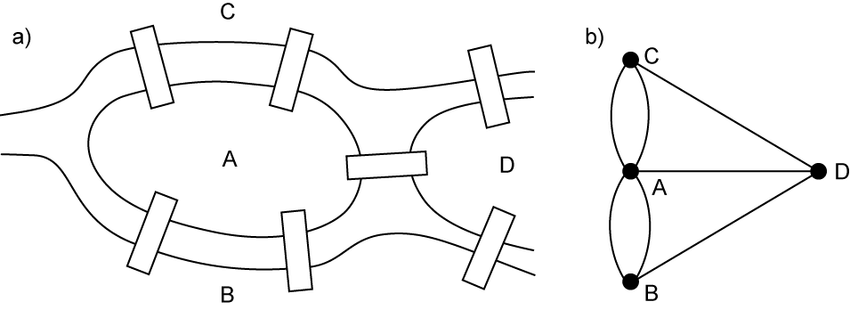
\includegraphics[scale=0.5]{Koenigsberg.png}
  \captionsetup{font=small,position=below,skip=-1pt}
   \caption*{Fonte: Boguslawski, Pawel \cite{Koenigsberg}.}
   \label{Konigsberg}
\end{figure}

A prova de Euler nos mostra que quando queremos modelar algum problema não é necessário considerar todas as variáveis existentes neles, mas o essencial para a solução. Nesse caso o mais importante foi esquematizar o problema usando Grafos e, principalmente, analisar uma estrutura intrínseca ao Grafo.

Com a solução do problema surge a área da matemática chamada Grafos que é a base matemática para o que chamamos em redes. Essa nomenclatura varia de área para área, na física, por exemplo, são sinônimos enquanto que na computação Grafos estão relacionados à problemas de fluxo \cite{Grafos01,Grafos} e Redes são utilizados para problemas visando a estrutura do Grafo e suas interações \cite{network,networks}. Nesse trabalho usaremos os dois como sinônimo.

\section{Conceitos Fundamentais}

Um Grafo $G(\mathpzc{N} ,\mathpzc{L})$ é uma dupla na qual $\mathpzc{N} = \{0,1,2,...,i,...\}$ é um conjunto não vazio de elementos chamados de vértices, ou nós, e $\mathpzc{L}$ é um conjunto não vazio de pares não ordenados de elementos de $\mathpzc{N}$. Dessa forma podemos definir $N = |\mathpzc{N}|$ que mensura a quantidade de vértice que há em $G$ e $L= |\mathpzc{L}|$ que mensura o número de arestas. Essas quantidades também são chamadas de ordem e tamanho \cite{Grafos}, respectivamente, que medem a cardinalidade de $\mathpzc{N}$ e $\mathpzc{L}$.

A partir dessa definição de redes podemos definir a Matriz de Adjacência, ela vai guardar a informação de quem está conectado com quem. Seja uma matriz A quadrada de tamanho $N \times N$, cada elemento da matriz segue a seguinte regra:
\[   
  a_{i,j} = 
     \begin{cases}
       1 \quad \text{se i e j estão conectados}\\
       0 \quad \text{caso contrário.} \\
     \end{cases}
\]

A partir dela surgem características importantes de redes. Se $a_{i,j} = a_{j,i} \forall i,j \in \mathpzc{N}$ então a rede é chamada de não direcionada, se $a_{i,j} \neq a_{j,i} \forall i,j \in \mathpzc{N}$ ela é chamada de direcionada. Isso pode ter diferentes interpretações a depender do contexto inserido. Por exemplo na rede de amigos do Facebook, se o usuário A é amigo de B, então B é amigo de A. No caso do Instagram se A segue B não necessariamente B segue A. No primeiro caso é natural modelarmos utilizando redes não direcionadas, enquanto que no segundo usamos redes direcionadas.

Uma outra forma de guardamos a informação de quem está conectado com quem é a partir da lista de vizinhos. Dois vértices $i$ e $j$ são vizinhos se existe uma ligação entre $i$ e $j$, assim denotamos $\nu(i)$ o conjunto de vizinhos do vértice $i$ para redes não direcionadas. Em redes direcionadas agora temos dois tipos de vizinhos $(i,j)$ e $(k,i)$, portanto denotaremos $\nu_{in}(i)$ todos os vizinhos que têm ligação que chega em $i$ e $\nu_{out}(i)$ todos os vizinhos que têm ligação que sai em $i$.

Por fim, podemos adicionar pesos às nossas ligações, isso têm várias interpretações nos problemas: em uma rede de canos de esgoto, o fluxo que passa em um cano pode ser um peso e em redes de Facebook o nível de amizade pode ser um peso das ligações entre usuários, dentre outros exemplos. Ou podemos adicionar aos vértices como em redes sociais se quisermos estudar a propagação de um vírus a idade ou se ela faz parte de um grupo de risco ou não são parâmetros importantes a serem analizados. Formalmente, um Grafo ponderado $G(\mathpzc{N},\mathpzc{L},\omega)$ é formado por um conjunto de Nós $\mathpzc{N}$, um conjunto de arestas $\mathpzc{L}$ e um mapeamento $\omega: \mathpzc{L}\mapsto \mathbb{R}$ e/ou $\omega: \mathpzc{N}\mapsto \mathbb{R}$. Nesse sentido podemos definir a matrix de pesos $W$ que apresenta uma definição parecida da Matriz de Adjacência, seja $T$ um valor limiar então:

\[   
  w_{i,j} = 
     \begin{cases}
       \omega(i,j) \quad \text{se i e j estão conectados e} \omega(i,j)> T\\
       0 \quad \text{caso contrário.} \\
     \end{cases}
\]

\section{Métricas de Redes}

Como discutido anteriormente é muito importante estudarmos a estrutura da rede, pois elas vão governar o comportamento da rede. Para entendermos melhor essa estrutura existem várias métricas \cite{Costa2007} relacionadas à topologia da rede podendo ser classificadas como globais ou locais. As métricas globais são aquelas que estão intrinsecamente ligada ao Grafo, enquanto que as locais estão ligadas à cada vértice da rede.

\subsection{Métricas Globais de Redes}

A primeira delas a ser analisada é a medida de distância entre um vértice e outro. Seja dois vértices $i,j \in \mathpzc{N}$ dizemos que existe um caminho entre $i$ e $j$ se existe uma sequência de vértices $\nu_1,\nu_2,...,\nu_k | (\nu_{s},\nu_{s+1}) \in \mathpzc{L} $ $\forall$ $ 1 \leq s < k $ e $\nu_1 = i,\nu_k = j$. Existem vários caminhos que podem existir entre $i$ e $j$, portanto a nossa distância geodésica entre dois vértices $l_{i,j}$ é definida como a quantidade de arestas do menor caminho entre $i,j$.

Agora que definimos qual é a distância em redes que usaremos, outras métricas surgem a partir dessa definição. Por exemplo temos o menor caminho médio de toda a rede:

\begin{equation}
  \left\langle l \right\rangle  = \sum_{\substack{i,j \\ i\neq j}} \frac{l_{i,j}}{N\cdot(N-1)}.
\end{equation}

Esse valor nos dá a informação sobre o quanto em média é necessário caminhar na rede de um nó para outro. Outro valor importante é o chamado diâmetro $d$ que é a maior distância geodésica da rede

\begin{equation}
  d = \max l_{i,j}
\end{equation}

Esses valores são bastante importantes para estudos em redes de pequeno mundo \cite{Kleinberg} na qual discutiremos nas próximas sessões.

Uma outra métrica a ser avaliada é quantas conexões cada nó contém. Definiremos o grau $k_i$ do nó $i$ como sendo o número de conexões (ou vizinhos) que o nó $i$ possui para redes não direcionadas. Para redes direcionadas teremos outra divisão entre $k^{in}_i$ e $k^{out}_i$ para os sítios que pertencem a $\nu_{in}(i)$ e $\nu_{out}(i)$. Podemos achar esses valores a partir da Matriz de Adjacência:

\begin{multicols}{2}
  \begin{equation*}
    k^{in}_i = \sum_{j} A_{ij}
  \end{equation*}
  \break
  \begin{equation}
    k^{out}_i = \sum_{j} A_{ji}.
  \end{equation}
\end{multicols}

Além disso podemos também definir o grau médio $\left\langle k \right\rangle$ da rede esse valor tem bastante importância quantitativa quando queremos trabalhar com distribuições de graus.

\begin{equation}
  \left\langle k \right\rangle = \sum_{i \in G}\frac{k_i}{N} = 2\frac{L}{N}
  \label{grau_tamanho}
\end{equation}

Outras duas métricas importantes são a densidade $\rho(G)$ e a reciprocidade $rc(G)$. A primeira mede a razão entre a quantidade de arestas dentro do grafo $G$ pela quantidade total de arestas que o grafo pode suportar. Já a segunda nos apresenta a fração de arestas que existem em ambas as direções, no caso trivial de redes não direcionadas esse valor é igual a 1.

\[   
  \rho(G) = 
     \begin{cases}
      \frac{2L}{N\cdot(N-1)} \quad \text{se a rede for não direcionada, ou }\\
      \frac{L}{N\cdot(N-1)} \quad \text{se a rede for direcionada.} \\
     \end{cases}
\]

\begin{equation}
  rc(G) = \frac{\sum_{i,j} A(i,j)A(j,i)}{\sum_{i,j} A(i,j)}
\end{equation}

Por fim temos uma métrica para analisar o Agrupamento de uma Rede, ou seja quanto que os vértices estão unidos. Essa métrica será definida a partir da probabilidade de um vizinho do nó $i$ estar conectado com outro vizinho de $i$. Existe a definição desse valor a partir da Matriz de Adjacência pela \ref{clustering1}, porém é mais compreensível compreensível pela \ref{clustering2}

\begin{equation}
  cl(G) = \frac{\sum_{(i,j,k): i\neq j \neq k}A(i,j)A(j,k)A(k,j)}{\sum_{(i,j,k): i\neq j \neq k}A(i,j)A(j,k)},
  \label{clustering1}
\end{equation}

\begin{equation}
  cl(G) = 3\frac{\#Triangulos}{\#Triades}.
  \label{clustering2}
\end{equation}

Em que 

\subsection{Métricas de Centralidade}

Ao estudar redes estamos interessados em entender suas estruturas e propriedades, isso já é possível dadas as métricas que apresentamos anteriormente. Contudo, essas métricas globais nos trazem informações sobre a rede como um todo e as propriedades que ela apresenta podem estar diluídas na rede como um todo ou concentrada em sítios específicos. Portanto estudar os sítios em si e a sua importância perante a rede é necessário, para isso usaremos as chamadas Métricas de Centralidade.

Centralidade nesse contexto está ligado à importância, quando falamos de Métricas de Centralidade queremos estudar a importância topológica de cada nó perante a rede. Mas em que sentido seria essa importância? Depende do problema, talvez seja necessário estudar qual o autor mais importante em uma rede de citações de artigos ou qual pessoa devemos retirar de uma rede social para inibir a propagação de \textit{fake-news} para ambas existe uma métrica apropriada para atingir tais objetivos.

A primeira métrica a ser avaliada é propriamente o número de conexões de cada sítio, o grau $k_i$. Ao avaliarmos essa métrica consideramos o sítio central aquele que tem o maior $k_i$, ou seja estamos atrás daquele sítio que apresenta mais ligações.

A segunda métrica importante é a Centralidade de Excentricidade (CE). Excentricidade está definido no dicionário como "desvio ou distância para o centro", no nosso caso a CE vai apontar qual sítio é mais central baseado na maior distância que o sítio pode percorrer na rede, sendo ele o mais central aquele que tem a menor distância máxima. Formalmente $CE(i) \forall i \in \mathpzc{N}$ é definida como:

\begin{equation}
  CE(i) = \frac{1}{\max_{\forall j \in \mathpzc{N}} l_{i,j}}
\end{equation}

Nessa mesma ideia podemos avaliar outras duas métricas parecidas: Centralidade de Proximidade (CP) e Centralidade Harmônica (CH). Em ambas estamos interessados a entender qual é o nó mais central a partir de quanto ele dista dos outros, a diferença entre as duas é que a primeira é calculado pelo inverso da média aritmética e a segunda com a média harmônica.

\begin{equation}
  CP(i) = \frac{N - 1}{\sum_{j \neq i} l_{i,j}}
\end{equation}

\begin{equation}
  CH(i) = \frac{1}{N - 1}\sum_{j \neq i}\frac{1}{l_{i,j}}
\end{equation}

\section{Modelos de Formação de Redes}

Na sessão anterior discutimos sobre as métricas que tentam quantificar a estrutura da rede, nesse sentido dada um grafo $G$ conseguimos extrair as suas propriedades. Contudo, será que seria possível fazer o contrário? Dado uma propriedade conseguimos criar uma Rede que contenha essas propriedades? Portanto, nessa sessão explicaremos os principais modelos utilizados para formarmos redes artificiais.

\subsection{Rede de Erdös-Rényi}

A Rede de Erdös-Rényi, ou rede aleatória, parte do princípio que nossas conexões com outras pessoas são aleatórias. Ao trabalharmos nesse modelo nós temos o conhecimento de quantos sítios e ligações existem

\subsection{Modelo de Configuração}

Diferente do Modelo de Erdös-Rényi podemos encontrar o caso na qual nós sabemos que o nosso grafo tem uma quantidade $N$ de sítios e sabemos qual a sequência de graus $\{k_i\}$ cada sítio $i$ da rede. Para gerar redes assim usamos o chamado Modelo de Configuração (MC). Esse modelo tem uma restrição de que o número de ligações (que pode ser obtido facilmente por \ref{grau_tamanho}) ser um número par. O modelo segue da seguinte forma:

\begin{enumerate}
  \item Criam-se os $N$ vértices da rede;
  \item Cada vértice $i$ recebe $\kappa_i$ ligações a serem criadas;
  \item Escolhemos o vértice $i$ em ordem decrescente de grau da sequência $\{\kappa_i\}$ (isso serve para facilitar a convergência do modelo);
  \item Escolhemos aleatoriamente outro $j$ sítio da rede que não tenha ligação com $i$ e que ainda não tenha criada todas as $\kappa_j$ ligações e criamos a ligação e reduzimos em 1 o valor de $\kappa_i$ e $\kappa_j$;
  \item Repetimos 3 e 4 até colocarmos todas as ligações na rede.
\end{enumerate}

\begin{algorithm}

  \caption{Modelo de Configuração}\label{alg:MC}
  \begin{algorithmic}
  \Require $k$ \Comment{Essa lista está em ordem decrescente de grau.}
  \Require $edges$\\

  \While{($i \in \mathpzc{N}$) and ($k_i \in k$)} \Comment{Os sítios são escolhidos em ordem decrescente de grau.}
    \State $\kappa_i \gets k_i$
    \While{$j \in \mathpzc{N}$}
      \If{($i \neq j$) and ($k_i \neq 0$)}
          \If{(i,j not in $edges$) and ($k_j \neq 0$)}
            \State $edges$.insert((i,j))
            \State $\kappa_i \gets \kappa_i - 1$
            \State $\kappa_j \gets \kappa_j - 1$
          \EndIf
      \EndIf
    \EndWhile
  \EndWhile
  \end{algorithmic}

\end{algorithm}

\begin{figure}[!h]
  \centering
  \captionsetup{font=normalsize,skip=0.8pt,singlelinecheck=on,labelsep=endash}
  \caption{Ilustração do Modelo}
  \begin{tikzpicture}
    \draw[gray, thick, dotted] (0,0) -- (-1,-1);
    \draw[gray, thick] (0,0) -- (1,1);
    \draw[gray, thick, dotted] (0,0) -- (1,-1);
    \draw[gray, thick, dotted] (0,0) -- (-1,1);
    \draw[black, fill=white] (0,0) circle [radius=0.25] node {$i$};
    \draw[gray, thick, dotted] (1,1) -- (2,2);
    \draw[gray, thick] (3,3) -- (2,2);
    \draw[gray, thick, dotted] (3,3) -- (4,2);
    \draw[gray, thick, dotted] (3,3) -- (2,4);
    \draw[black, fill=white] (3,3) circle [radius=0.25] node {$j$};
  
    \draw[gray, thick, dotted] (0,3) -- (0,2);
    \draw[gray, thick, dotted] (0,3) -- (0,4);
    \draw[gray, thick, dotted] (0,3) -- (-1,3);
    \draw[gray, thick, dotted] (0,3) -- (1,3);
    \draw[black, fill=white] (0,3) circle [radius=0.25] node {9};
  
    \draw[gray, thick, dotted] (3,0) -- (4,-1);
    \draw[gray, thick, dotted] (3,0) -- (2,-1);
    \draw[black, fill=white] (3,0) circle [radius=0.25] node {3};
    
    %\filldraw (0,0) circle (7pt) node[anchor=west, inner sep=0pt]{i};
  \end{tikzpicture}
  \captionsetup{font=small}
  \caption{Funcionamento do Modelo de Configuração, escolhemos dois sítios $i$ e $j$ aleatoriamente e os conectamos. Fonte: Elaborado pelo autor}
  \label{img:MC}
\end{figure}

\section{Modelos de Infecção}

%%%%%%%%%%%%%%%%%%%%%%%%%%%%%%%RECOMENDACAO%%%%%%%%%%%%%%%%%%%%%%%%%%
% faca os capitulos separados, não coloque \documentclass{} e \begin{document} \end{document}
% EX: no cap1.tex coloque:
% \chapter{titulo do capitulo} sem numerar, isso e feito automaticamente pelo LaTeX


%\include{cap1}
%\include{cap2}
%\include{cap3}
\chapter{Metodologia}

Por conseguinte é natural a utilização de Redes Complexas como modelagem para estudos da Covid-19. Para tanto precisamos agora de dados sobre redes de contágio que contenham informações relevantes para esse estudo, como idade, tempo de contato, se faz parte de grupo de risco ou não, dentre outros.

Entretanto, não é fácil encontrar um banco de dados tão completo assim e não enviesado pela recente pandemia. Em 2008, visando o estudo da pandemia de influenza a Comissão Europeia criou o projeto chamado POLYMOD \cite{POLYMOD} que tinha o intuito da coleta de dados para entender como quais seriam os padrões de contatos da Europa \cite{Mossong2008}.

Apoiado nesse estudo, pesquisas posteriores se inspiraram no molde do POLYMOD \cite{Belga2009,Belga2010,China,France,HongKong,Peru,Russia,Thailand,Vietnam,Zambia,Zimbabwe}. Apesar da grande quantidade de pessoas e contatos há um problema essencial: não há garantia de que as pessoas da entrevista se conectem em si. Por exemplo, no caso da França \cite{France} foram feitas ligações aleatórias extraída da população francesa excluindo territórios ultramarinos, assim nossa análise em rede estaria bastante limitada.

Para evitar esse problema \cite{Manzo2020} propõe um modelo para formamos uma rede baseado nos dados franceses. A partir dos dois dias de entrevista é calculado a média de contatos por dia de cada pessoa (arredondado para cima) e utiliza o Modelo de Configuração para a formação de uma Rede Sintética. No entanto, o modelo de formação de redes gera um agrupamento médio limitado e ele é muito importante na suavização de epidemias \cite{Block2020}. Nesse sentido Manzo propõe que antes de excluirmos um dado sítio do Modelo de Configuração, passamos por cada vizinho dele e os conectamos entre si com uma probabilidade $p$. Ou seja:

\begin{enumerate}
  \item Quando um dado sítio $i$ atinge o grau requerido pelo MC selecionamos todos os vizinhos $\nu(i)$;
  \item Selecionamos dois sítios $v,n \in \nu(i)$ e conectamos com probabilidade $p$;
  \item Se ela existir os conectamos e salvamos para que ela não se repita no MC, caso contrário salvamos para que ela não se repita nesse algoritmo. Por fim também reduzimos em 1 o valor de $\kappa_v$ e $\kappa_n$ ;
  \item Fazemos 2. até testarmos todas as ligações possíveis e paramos esse algoritmo para dar continuidade ao MC.
\end{enumerate}

\begin{algorithm}

  \caption{Implementação de Manzo}\label{alg:cap}
  \begin{algorithmic}
  \Require $edges$
  \Require $\kappa$
  \Require $n\_existir$ \Comment{É necessário salvar quais ligações não vão existir.}
  \Require $p$
  \Require $i \in G(\mathpzc{N} ,\mathpzc{L})$\\

  \While{$v \in \nu(i)$}
    \While{$n \in \nu(i)$} \Comment{Nesse caso não há preferência na escolha de $n$ e $v$.}
      \If{($v \neq n$) and ($\kappa_n \neq 0$) and ($\kappa_v \neq 0$)}
          \State $r$ $\gets$ random\_number([0,1])
          \If{($r <= p$)}
            \If{($v,n$ not in $edges$) and ($v,n$ not in $n\_existir$)}
              \State $edges$.insert(($v,n$)) \Comment{Essa matriz vem do MC}
              \State $\kappa_v \gets \kappa_v - 1$
              \State $\kappa_n \gets \kappa_n - 1$
            \EndIf
          \Else
          \If{$n,v$ not in $n\_existir$}
            \State $n\_existir$.insert((v,n))
            \EndIf
          \EndIf
      \EndIf
    \EndWhile
  \EndWhile
  \end{algorithmic}

\end{algorithm}

\begin{figure}[!h]
  \centering
  \captionsetup{font=normalsize,skip=0.8pt,singlelinecheck=on,labelsep=endash}
  \caption{Ilustração do Modelo de Manzo}
  \begin{tikzpicture}[make origin horizontal center of bounding box]
    %Values
    \def\xa{2};
    \def\ya{sqrt(4-sqrt(\xa))}

    \def\xc{0.5};
    \def\yc{sqrt(4-sqrt(\xc))};

    \def\xb{0.5};
    \def\yb{sqrt(4-sqrt(\xb))};

    \def\xd{1.5};
    \def\yd{sqrt(4-sqrt(\xd))};

    \def\xe{1.3};
    \def\ye{sqrt(4-sqrt(\xe))};

    \draw[black, thick] (0,0) -- ($\xa*(1,0) + \ya*(0,1)$);

    \draw[black, thick, dotted]($\xa*(1,0) + \ya*(0,1)$) -- ($\xa*(0.5,0) + \ya*(0,0.01)$);

    
    \draw[black, thick] (0,0) -- ($\xb*(1,0) + \yb*(0,1)$);
    \draw[black, thick, dotted] ($\xb*(1,0) + \yb*(0,1)$) -- ($\xb*(1,0) + \yb*(0,1.5)$);
    \draw[black, thick, dotted] ($\xb*(1,0) + \yb*(0,1)$) -- ($\xa*(1,0) + \ya*(0,1)$);
    \draw[black, thick, dotted] ($\xb*(1,0) + \yb*(0,1)$) -- ($\xc*(1,0.5) + \yc*(0.3,0.5)$);
    \draw[black, thick, dotted] ($\xb*(1,0) + \yb*(0,1)$) -- ($\xc*(1,0.5) + \yc*(-0.3,0.5)$);

    \draw[black, thick] (0,0) -- ($\xc*(1,0) + \yc*(0,-1)$);
    \draw[black, thick, dotted] ($\xc*(1,0) + \yc*(0,-1)$) -- ($\xa*(0.7,0) + \ya*(0,0.01)$);
    \draw[black, thick, dotted] ($\xc*(1,0) + \yc*(0,-1)$) -- ($\xc*(-1.5,0) + \yc*(0,-1)$);
    

    \draw[black, thick] (0,0) -- ($\xd*(-1,0) + \yd*(0,-1)$);
    \draw[black, thick, dotted] ($\xd*(-1,0) + \yd*(0,-1)$) -- ($\xd*(-1,0) + \yd*(0,0.01)$);
    \draw[black, thick, dotted] ($\xd*(-1,0) + \yd*(0,-1)$) -- ($\xd*(-1.8,0) + \yd*(0,-1)$);

    \draw[black, thick] (0,0) -- ($\xe*(0,1) + \ye*(-1,0)$);

    % Nós

    \draw[black, fill=white, anchor=center] (0,0) circle [radius=0.25] node {3};
    \draw[black, fill=white] ($\xc*(1,0) + \yc*(0,1)$) circle [radius=0.25] node {5};
    \draw[black, fill=white] ($\xe*(0,1) + \ye*(-1,0)$) circle [radius=0.25] node {0};
    \draw[black, fill=white] ($\xd*(-1,0) + \yd*(0,-1)$) circle [radius=0.25] node {80};
    \draw[black, fill=white] ($\xb*(1,0) + \yb*(0,-1)$) circle [radius=0.25] node {32};
    \draw[black, fill=white] ($\xa*(1,0) + \ya*(0,1)$) circle [radius=0.25] node {18};
    \node at (0,3) {$p = 0$};
  \end{tikzpicture}
  \begin{tikzpicture}[make origin horizontal center of bounding box]
    %Values
    \def\xa{2};
    \def\ya{sqrt(4-sqrt(\xa))}

    \def\xc{0.5};
    \def\yc{sqrt(4-sqrt(\xc))};

    \def\xb{0.5};
    \def\yb{sqrt(4-sqrt(\xb))};

    \def\xd{1.5};
    \def\yd{sqrt(4-sqrt(\xd))};

    \def\xe{1.3};
    \def\ye{sqrt(4-sqrt(\xe))};

    \draw[black, thick] (0,0) -- ($\xa*(1,0) + \ya*(0,1)$);

    \draw[black, thick, dotted]($\xa*(1,0) + \ya*(0,1)$) -- ($\xa*(0.5,0) + \ya*(0,0.01)$);

    
    \draw[black, thick] (0,0) -- ($\xb*(1,0) + \yb*(0,1)$);
    \draw[black, thick, dotted] ($\xb*(1,0) + \yb*(0,1)$) -- ($\xb*(1,0) + \yb*(0,1.5)$);
    \draw[black, thick] ($\xb*(1,0) + \yb*(0,1)$) -- ($\xa*(1,0) + \ya*(0,1)$);
    \draw[black, thick, dotted] ($\xb*(1,0) + \yb*(0,1)$) -- ($\xc*(1,0.5) + \yc*(0.3,0.5)$);
    \draw[black, thick, dotted] ($\xb*(1,0) + \yb*(0,1)$) -- ($\xc*(1,0.5) + \yc*(-0.3,0.5)$);

    \draw[black, thick] (0,0) -- ($\xc*(1,0) + \yc*(0,-1)$);
    \draw[black, thick, dotted] ($\xc*(1,0) + \yc*(0,-1)$) -- ($\xa*(0.7,0) + \ya*(0,0.01)$);
    %\draw[black, thick, dotted] ($\xc*(1,0) + \yc*(0,-1)$) -- ($\xc*(-1.5,0) + \yc*(0,-1)$);
    

    \draw[black, thick] (0,0) -- ($\xd*(-1,0) + \yd*(0,-1)$);
    \draw[black, thick] ($\xd*(-1,0) + \yd*(0,-1)$) -- ($\xc*(1,0) + \yc*(0,-1)$);
    \draw[black, thick, dotted] ($\xd*(-1,0) + \yd*(0,-1)$) -- ($\xd*(-1.8,0) + \yd*(0,-1)$);

    \draw[black, thick] (0,0) -- ($\xe*(0,1) + \ye*(-1,0)$);

    % Nós

    \draw[black, fill=white, anchor=center] (0,0) circle [radius=0.25] node {3};
    \draw[black, fill=white] ($\xc*(1,0) + \yc*(0,1)$) circle [radius=0.25] node {5};
    \draw[black, fill=white] ($\xe*(0,1) + \ye*(-1,0)$) circle [radius=0.25] node {0};
    \draw[black, fill=white] ($\xd*(-1,0) + \yd*(0,-1)$) circle [radius=0.25] node {80};
    \draw[black, fill=white] ($\xb*(1,0) + \yb*(0,-1)$) circle [radius=0.25] node {32};
    \draw[black, fill=white] ($\xa*(1,0) + \ya*(0,1)$) circle [radius=0.25] node {18};
    \node at (0,3) {$p = 0.5$};
  \end{tikzpicture}
  \begin{tikzpicture}[make origin horizontal center of bounding box]
    %Values
    \def\xa{2};
    \def\ya{sqrt(4-sqrt(\xa))}

    \def\xc{0.5};
    \def\yc{sqrt(4-sqrt(\xc))};

    \def\xb{0.5};
    \def\yb{sqrt(4-sqrt(\xb))};

    \def\xd{1.5};
    \def\yd{sqrt(4-sqrt(\xd))};

    \def\xe{1.3};
    \def\ye{sqrt(4-sqrt(\xe))};

    \draw[black, thick] (0,0) -- ($\xa*(1,0) + \ya*(0,1)$);

    %\draw[black, thick, dotted]($\xa*(1,0) + \ya*(0,1)$) -- ($\xa*(0.5,0) + \ya*(0,0.01)$);

    
    \draw[black, thick] (0,0) -- ($\xb*(1,0) + \yb*(0,1)$);
    \draw[black, thick, dotted] ($\xb*(1,0) + \yb*(0,1)$) -- ($\xb*(1,0) + \yb*(0,1.5)$);
    \draw[black, thick] ($\xb*(1,0) + \yb*(0,1)$) -- ($\xa*(1,0) + \ya*(0,1)$);
    \draw[black, thick, dotted] ($\xb*(1,0) + \yb*(0,1)$) -- ($\xc*(1,0.5) + \yc*(0.3,0.5)$);
    %\draw[black, thick, dotted] ($\xb*(1,0) + \yb*(0,1)$) -- ($\xc*(1,0.5) + \yc*(-0.3,0.5)$);

    \draw[black, thick] (0,0) -- ($\xc*(1,0) + \yc*(0,-1)$);
    %\draw[black, thick, dotted] ($\xc*(1,0) + \yc*(0,-1)$) -- ($\xa*(0.7,0) + \ya*(0,0.01)$);
    %\draw[black, thick, dotted] ($\xc*(1,0) + \yc*(0,-1)$) -- ($\xc*(-1.5,0) + \yc*(0,-1)$);
    

    \draw[black, thick] (0,0) -- ($\xd*(-1,0) + \yd*(0,-1)$);
    \draw[black, thick] ($\xd*(-1,0) + \yd*(0,-1)$) -- ($\xc*(1,0) + \yc*(0,-1)$);
    \draw[black, thick] ($\xd*(-1,0) + \yd*(0,-1)$) -- ($\xb*(1,0) + \yb*(0,1)$);
    \draw[black, thick] ($\xb*(1,0) + \yb*(0,-1)$) -- ($\xa*(1,0) + \ya*(0,1)$);

    \draw[black, thick] (0,0) -- ($\xe*(0,1) + \ye*(-1,0)$);

    % Nós

    \draw[black, fill=white, anchor=center] (0,0) circle [radius=0.25] node {3};
    \draw[black, fill=white] ($\xc*(1,0) + \yc*(0,1)$) circle [radius=0.25] node {5};
    \draw[black, fill=white] ($\xe*(0,1) + \ye*(-1,0)$) circle [radius=0.25] node {0};
    \draw[black, fill=white] ($\xd*(-1,0) + \yd*(0,-1)$) circle [radius=0.25] node {80};
    \draw[black, fill=white] ($\xb*(1,0) + \yb*(0,-1)$) circle [radius=0.25] node {32};
    \draw[black, fill=white] ($\xa*(1,0) + \ya*(0,1)$) circle [radius=0.25] node {18};
    \node at (0,3) {$p = 1$};
  \end{tikzpicture}
  \captionsetup{font=small}
  \caption{Funcionamento do Modelo de Configuração, escolhemos dois sítios $i$ e $j$ aleatoriamente e os conectamos. O Algoritmo pode gerar várias topologias de redes, porém ainda limitadas pelas quantidades $\{k_i\}$ de graus impostas pelo MC.\\ Fonte: Elaborado pelo autor}
  \label{img:MC_P}
\end{figure}

O Modelo é mostrado na Figura \ref{img:MC_P}, na qual mostramos o estágio quando encontramos um dado sítio que atinge o grau especificado. Assim como nos modelos de formação de rede existem várias redes que podem ser formadas dada uma probabilidade $p$. Outrossim, se o sítio já tiver atingido o grau requerido pelo MC, então ele não precisa entrar nesse algoritmo. A partir desse modelo o autor consegue os seguintes resultados mostrados na Tabela \ref{table:Manzo} e os meus estão na Tabela \ref{table:Miguel}.

\begin{table}[H]
  \centering
  \captionsetup{margin={9pt,14pt},font=normalsize,skip=0.5pt,labelsep=endash}

  \caption{Tabela do resultado de Manzo}
  \hspace*{-\leftmargin}\begin{tabular}{lccccccc}

    \hline

    \multicolumn{1}{l|}{ \textbf{\shortstack{Probabi\\-lidade}}} & 
    \multicolumn{1}{c|}{\textbf{\shortstack{Grau \\ Médio}}}  & 
    \multicolumn{1}{c|}{\textbf{\shortstack{Grau \\ Mediano}}} &
    \multicolumn{1}{c|}{\textbf{\shortstack{Desvio \\ Padrão \\ Grau}}} &
    \multicolumn{1}{c|}{\textbf{\shortstack{Agrupa-\\mento \\ Médio}}} & 
    \multicolumn{1}{c|}{\textbf{\shortstack{Corr \\ Agrup-\\ Grau}}} & 
    \multicolumn{1}{c|}{\textbf{\shortstack{Menor \\ Caminho \\ Médio}}} & 
    \multicolumn{1}{c}{{\shortstack{\textbf{Diâmetro}}}}     \\

    \hline\\
    \rowcolor{Gray}
p = 0         & 9.72 (0.00) & 8 (0.00)     & 6.56 (0.00)        & 0.01 (0.00)       & -0.06 (0.01)                  & 3.47 (0.00)         & 6 (0.00)     \\
  p = 0.5       & 9.72 (0.00) & 8 (0.00)     & 6.56 (0.00)        & 0.43 (0.00)       & -0.62 (0.01)                  & 4.38 (0.03)         & 7.45 (0.5)   \\
  \rowcolor{Gray}
  p = 1.0       & 9.72 (0.00) & 8 (0.00)     & 6.56 (0.00)        & 0.57 (0.01)       & -0.56 (0.01)                  & 5.52 (0.09)         & 10.10 (0.59)

  
\end{tabular}

  \captionsetup{margin={10pt,10pt},font=small,skip=0pt,position=below}

  \caption*{Aqui aparece os resultados advindos do autor para a rede francesa feitas em 100 simulações de redes. Apresentando as características da rede e em parêntese o erro associado a cada valor. \\Fonte: Elaborada pelo autor.}
\label{table:Manzo}
\end{table}

Os valores com probabilidade $p = 0$ batem perfeitamente com os resultados do autor, os outros valores se aproximam bastante do que aparece no artigo, porém ainda na mesma faixa de erro. Podemos ver que o Grau permanece o mesmo para que seja respeitado o MC já o agrupamento aumenta bastante com o incremento de $p$ chegando a seu valor máximo em $0.56$ que é limitado pelo MC.

\begin{table}[H]
  \centering
  \captionsetup{margin={9pt,14pt},font=normalsize,skip=0.5pt,labelsep=endash}

  \caption{Tabela do meu resultado.}
  \hspace*{-\leftmargin}\begin{tabular}{lccccccc}

    \hline

    \multicolumn{1}{l|}{ \textbf{\shortstack{Probabi\\-lidade}}} & 
    \multicolumn{1}{c|}{\textbf{\shortstack{Grau \\ Médio}}}  & 
    \multicolumn{1}{c|}{\textbf{\shortstack{Grau \\ Mediano}}} &
    \multicolumn{1}{c|}{\textbf{\shortstack{Desvio \\ Padrão \\ Grau}}} &
    \multicolumn{1}{c|}{\textbf{\shortstack{Agrupa-\\mento \\ Médio}}} & 
    \multicolumn{1}{c|}{\textbf{\shortstack{Corr \\ Agrup-\\ Grau}}} & 
    \multicolumn{1}{c|}{\textbf{\shortstack{Menor \\ Caminho \\ Médio}}} & 
    \multicolumn{1}{c}{{\shortstack{\textbf{Diâmetro}}}}     \\

    \hline\\\rowcolor{Gray}
    p = 0 & 9.72(0.00) & 8.00(0.00) & 6.56(0.00) & 0.01(0.00) & -0.06(0.01) & 3.47(0.00) & 6.00(0.03)  \\
p = 0.5                             & 9.72(0.00)                      & 8.00(0.00)   & 6.56(0.00)         & 0.43(0.01)        & -0.62(0.01)                   & 4.37(0.05)          & 7.46(0.50)  \\
p = 1.0                             & 9.72(0.00)                      & 8.00(0.00)   & 6.56(0.00)         & 0.56(0.01)        & -0.57(0.01)                   & 5.62(0.11)          & 10.39(0.66)

  
\end{tabular}

  \captionsetup{margin={10pt,10pt},font=small,skip=0pt,position=below}

  \caption*{Aqui aparece os resultados advindos do meu código na qual foram feitas 1000 simulações de redes para a rede francesa que se aproximam bastante do apresentado no artigo junto com os desvios padrões entre parênteses. Os que não bateram certo estão na faixa de erro mostrada anteriormente. \\Fonte: Elaborada pelo autor.}
\label{table:Miguel}
\end{table}



\newpage
\mycomment{


\begin{table}[h]
  \centering
\captionsetup{margin={9pt,14pt},font=normalsize,skip=0.5pt,labelsep=endash}
\caption{Distribui\c c\~ao dos documentos analisados por programa de p\'os-gradua\c c\~ao}
        \begin{tabular}{l|c|c|c}
           %\specialrule{1pt}{0pt}{0pt}
%    \multirow{2}{*}{\textbf{Programas de p\'os-gradua\c{c}\~ao~~~~~~~}}
    & \multicolumn{2}{c|}{\textbf{Categoria}}  &  \multirow{2}{*}{\textbf{~Total~}} \\
            \cline{2-3}
             & \textbf{~~~~~Teses~~~~~} & \textbf{Disserta\c{c}\~oes} &  \\
            \hline
            Cirurgia  & 1 & 1 & 2 \\
            Enfermagem & 4 &4 & 8 \\
            Engenharia Civil & 2 & 8 & 10 \\
            Farmacologia & 8 & 6 & 14 \\
            F\'isica & 3 & 6 & 9 \\
            Qu\'imica Inorg\^anica & 4 &1 & 5 \\
            {\bf Total}   & {\bf 22} & {\bf 26} & {\bf 48} \vspace{-0.6mm}\\ \bottomrule[1pt]
        \end{tabular}
\captionsetup{margin={10pt,10pt},font=small,skip=0pt,position=below}
\caption*{Fonte: Elaborada pelo autor.}
\end{table}

\begin{figure}[h]
\centering
\captionsetup{font=normalsize,skip=1pt,singlelinecheck=on,labelsep=endash}
\caption{Figura teste}

\includegraphics[scale=0.5]{ufc.jpg}
\captionsetup{font=small,position=below,skip=-1pt}
 \caption*{Fonte: Lara e Smit.}
 \label{fig1}
\end{figure}

\vskip2cm


\begin{grafico}[h]
\centering
\captionsetup{font=normalsize,skip=0.8pt,singlelinecheck=on,labelsep=endash}
\caption{Grafico de teste}

\includegraphics[scale=0.5]{ufc.jpg}
\vspace{-0,15cm}
\captionsetup{font=small}
  \caption*{Fonte: Elaborado pelo autor.}
  \label{graf1}
\end{grafico}
\newpage
\begin{grafico}[h]
\centering
\captionsetup{font=normalsize,skip=0.8pt,singlelinecheck=on,labelsep=endash}
\caption{Grafico de teste2}

\includegraphics[scale=0.5]{ufc.jpg}
\vspace{-0,15cm}
\captionsetup{font=small}
  \caption*{Fonte: Elaborado pelo autor.}
  \label{graf2}
\end{grafico}

}
\chapter{conclus\~ao}
% \begin{figure}[h]
% 
% \center
% \subfigure{\includegraphics[width=0.45\textwidth]{Potentials135-D=5,10-FermionRight-caso2-eta1.pdf}} 
% \qquad
% \subfigure{\includegraphics[width=0.45\textwidth]{T135-D=5,10-FermionRight-caso2-eta1.pdf}}
% \caption{Potentials $U(z)$ and Transmission coefficient $T(m^2)$ for massive right fermions (odd dimensions) and Dirac fermions (even dimensions choosing $\xi_{n+}(x)$)
% with $\lambda=0,4$ for $D=5$ (line) and $D=10$ (dotted), with $\eta=1$, $M=1$ and $s=1$ (a, d), $s=3$ (b, e) and $s=5$ (c, f).}
% \label{Potentials3}
% \end{figure}

%\include{apenda}
%%%USAR BIBITEX
\bibliography{exemplo.bib}
% \begin{thebibliography}{5}
% \bibitem{weinberg:cosmology}
%   S.~Weinberg,
%    {\it Cosmology},
%   Oxford University Press Inc., New York (2008)
%  \end{thebibliography}

%%%%ATENÇÃO!!!!!
%%OS APÊNDICES E ANEXOS DEVER VIR DEPOIS DAS REFERÊNCIAS
%%USAR COMANDO \achapter ao invés de \chapter. SEÇÕES CONTINUAM COM COMANDOS NORMAIS
\apendice
\achapter{Testando o apêndice}
\section{Teste}
\subsection{teste}
\achapter{teste2}
\section{teste}
\anexo
\achapter{Testando o anexo}
\end{document}
